% Preamble
\documentclass[14pt]{article}
%encoding
%--------------------------------------
\usepackage[T1]{fontenc}
\usepackage[utf8]{inputenc}
\usepackage[portuguese]{babel}
\usepackage{hyphenat}
\usepackage{fancyhdr}
\usepackage{graphicx}
\usepackage{float}
\usepackage{geometry}
\usepackage{hyperref}
\usepackage{imakeidx}
\usepackage{wrapfig}
\usepackage{lipsum}

\geometry{
a4paper,
total={170mm,257mm},
left=20mm,
top=20mm,
}

\hyphenation{mate-mática recu-perar}


\pagestyle{fancy}
\fancyhf{}
\fancyhead[LE,RO]{AED}
\fancyhead[RE,LO]{AirRoutes}
\fancyfoot[RE,CO]{António Vidais \and Tiago Leite}
\fancyfoot[LE,RO]{\thepage}
\graphicspath{ {images/} }
%--------------------------------------
\title{AirRoutes - Algoritmos e Estruturas de Dados}
\date{Dezembro de 2020}
\author{António Vidais \\96162 \and Tiago Leite \\96332}
% Document
\begin{document}
    \begin{titlepage}
        \begin{center}

            
\includegraphics[width=0.4\textwidth]{IST_logo.png}\\
            \vspace{0.5cm}
            Mestrado Integrado em Engenharia Eletrótecnica e de Computadores\\
            Instituto Superior Técnico\\
            1ºSemestre 2020\\
            Algoritmos e Estruturas de Dados\\
            \vspace*{1.5cm}
            \Huge
            \textbf{Projeto AirRoutes}
            \vspace{0.5cm}
            Grupo 32\\

                \vfill
                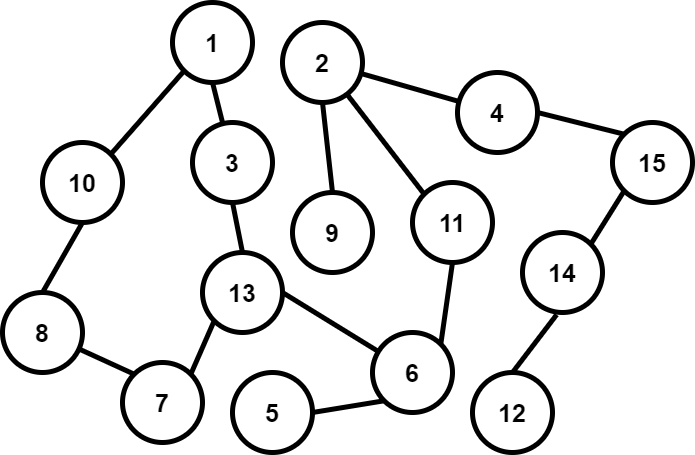
\includegraphics[width=1\textwidth]{15020D.png}
                \vfill
            \Large
            \textbf{António Vidais (96162) e Tiago Leite (96332)}\\
            \textbf{Professor Carlos Bispo}
        \end{center}
    \end{titlepage}

    \index{Indíce}

    \section{Descrição do Problema} \label{sec:d.problema}
    Este projeto, criado no âmbito da Unidade Curricular de Algoritmos e Estruturas de Dados, aborda o problema de
    encontrar um conjunto mínimo de rotas que garantam a existência de um caminho entre cada par de aeroportos,
    sem qualquer redundância.
    O Programa que este projeto visa produzir deve não só produzir uma rede mínima de rotas, mas sim a rede que garante
    todos os destinos já existentes, com o menor custo.
    Uma ferramenta como esta pode ser necessária, em termos práticos, quando uma companhia aérea quer ou precisa de otimizar de custos.
    Numa situação desta natureza, poderá ser necessário reduzir o seu conjunto de rotas à rede que
    garante que todos os aeroportos nela podem ser utilizados, com o menor custo.

    O Projeto que este relatório descreve foi desenvolvido na linguagem C, com recurso a Makefile e  e, para o seu correto funcionamento deve
    receber as informações de todas as rotas existentes através de um ficheiro de texto.
    Este deve conter uma ou mais redes de aeroportos, cada uma devidamente identificada com um cabeçalho contendo o
    número de aeroportos, o número total de rotas existentes e a variante que se pertende obter.
    Terminada a execução, o programa produz um segundo ficheiro de texto que contêm o conjunto mínimo de menor custo
    para cada rede fornecida, também identificados pelo cabeçalho fornecido, com a adição de algumas informações úteis,
    como o número de rotas mantidas e o custo total da rede

    \section{Abordagem do Problema}\label{sec:abordagem.problema}
    O Estudo de grafos assenta em alguns conceitos chaves, como o número de vértices (V), o número de arestas que ligam
    esses vértices (E), se as arestas são ponderadas (Custo) ou direcionadas, e a sua densidade (esparso ou denso).
    Para resolver este problema, foi necessário criar uma estrutura capaz de guardar uma representação do grafo formado
    pelo conjunto de rotas fornecido.
    A escolha desta estrutura requer uma análise cuidada ao tipo de grafo (denso ou esparço)e aos algoritmos que se
    pretende utilizar.
    Uma má escolha poderia levar a tempos de execução muito maiores que os pretendidos e maior utilização de memória,
    devido ao aumento da complexidade.

    \section{Arquitetura do Projeto}\label{arquitetura.projeto}
    A estrutura geral do programa é apresentada na Figura \ref{fig:main.flowchart}.
    Após verificar e inicializar os ficheiros necessários, procede-se à leitura dos Argumentos.
    Dependendo da leitura dos argumentos, é decidida a melhor forma de representação do grafo para o problema
    em questâo.
    As formas de representação do grafo são definidas com maior detalhe na secção\ref{sec:formas.representar.grafo}.

    \begin{figure}[H]
        \centering
        \label{fig:main.flowchart}
        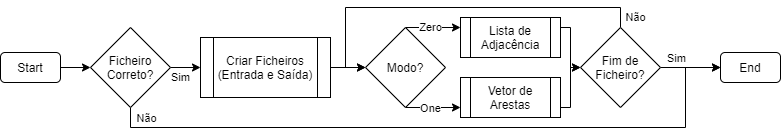
\includegraphics[scale=0.45]{main.flowchart.png}
        \caption{Fluxograma Representativo da execução da função main}
    \end{figure}

    \newpage

    \section{Estruturas e Tipos de Dados}\label{sec:estruturas.tipos.dados}

    \subsection[PBArg]{Argumentos do Problema}\label{subsec:argumentos.problema}
    A estrutura do tipo PBArg é usada para guardar os argumentos do problema. È declarada no ficheiro \emph{Graph.h}.
    Esta Estrutura é composta por:
    \begin{itemize}
        \item v : Integer que guarda o número de vértices no grafo;
        \item e : Integer que guarda o número de arestas no grafo;
        \item vi : Integer que guarda o 1º vértice da aresta a eliminar, nos modos aplicáveis;
        \item vj : Integer que guarda o 2º vértice da aresta a eliminar, nos modos aplicáveis;
        \item var : String que guarda a variante do problema pretendida;
        \item err : Boolean que é ativada quando ocorrem erros durante a execução;
    \end{itemize}

    \subsection[edge]{Aresta}\label{subsec:aresta}
    A estrutura do tipo Aresta é usada para guardar uma aresta, quer durante a sua leitura em ambos os modos, quer na
    sua manipulação no modo 1, onde está inserida na estrutura graph, para formar o vetor de arestas. Apesar de
    relativamente simples, esta estrutura é a base sobre a qual a maioria das funções deste programa operam. Por esse
    motivo foi propositamente tornada mais simples e eficiente.
    Esta Estrutura é composta por:
    \begin{itemize}
        \item vi : Integer que guarda o 1º Vértice da Aresta
        \item vj : Integer que guarda o 2º Vértice da Aresta
        \item cost : double que guarda o custo da aresta
    \end{itemize}

    \subsection[list]{Lista de Adjacências}\label{subsec:l.adj}
    A estrutura do tipo Lista de Adjacências é utilizada pelas funções do modo 0.
    Esta é a base para a representação do grafo sob a forma de vetor de listas de adjacências.
    As razões pelas quais esta representação do grafo foi escolhida para o modo 0 será discutida n\ref{subsec:formas.represent.grafo}.
    Esta Estrutura é composta por:
    \begin{itemize}
        \item v : Integer que guarda o vértice base da lista, a partir do qual se encontram os adjacentes;
        \item cost : Double que guarda o custo da aresta entra o vértice e o 1º vértice adjacente;
        \item next : Apontador para list que guarda o próximo elemento da lista;
    \end{itemize}

    \subsection[graph0]{Grafo sob a forma de Lista de Adjacência}\label{subsec:grafo.l.adj}
    A estrutura do tipo graph0 é a estrutura mãe para a representação do grafo na forma de listas de adjacências.
    Decidiu-se anexar à representação propriamente dita um apontador para \nameref{subsec:argumentos.problema} para
    facilitar grande parte dos parâmetros de entrada das funções.
    Assim, os \ref{subsec:argumentos.problema} são enviados em conjunto com a representação do grafo.
    Esta Estrutura é composta por:
    \begin{itemize}
        \item Arg : Estrutura do tipo \nameref{subsec:argumentos.problema} que guarda os argumentos referentes ao grafo
        representado no outro membro desta estrutura;
        \item data : Vetor de estruturas do tipo \nameref{subsec:l.adj} que guarda a lista de adjacências de todos os
        vértices do grafo;
    \end{itemize}

    \subsection[graph]{Grafo sob a forma de Vetor de Arestas}\label{subsec:grafo.v.are}
    A estrutura do tipo graph é a estrutura mãe da representação do grafo na forma de vetor de arestas.
    Como a estrutura \nameref{subsec:grafo.l.adj}, a estrutura \nameref{subsec:grafo.v.are} inclui um apontador para uma estrutura
    do tipo \nameref{subsec:argumentos.problema} para facilitar os parâmetros de entrada de grande parte das funções que operam
    sobre o grafo.
    Esta Estrutura é composta por:
    \begin{itemize}
        \item Arg : Estrutura do tipo \nameref{subsec:argumentos.problema} que guarda os argumentos referentes ao grafo apontado pelo vetor de arestas;
        \item data : Vetor de estruturas do tipo \nameref{subsec:aresta} que guarda todas as arestas lidas do ficheiro de entrada para o grafo em estudo;
    \end{itemize}

    \subsection[represent]{Formas de Representar o Grafo}\label{subsec:formas.representar.grafo}
    Para a resolução do Problema anteriormente discutido, decidiu-se representar o grafo sob a forma de \underline{Vetor de Arestas}.
    Nesta decisão, foram tidos em conta os seguintes fatores:
    \begin{itemize}
        \item O Ficheiro de Entrada é sempre um vetor de arestas;
        \item A leitura do ficheiro de entrada tem uma complexidade inerente mínima de E (Precorrer o grafo);
        \item O Algoritmo de \emph{Kruskal} recebe dados sob a forma de vetor de arestas. A escolha do Algoritmo de \emph{Kruskal} será discutida na secção \ref{sec:algoritmos}
    \end{itemize}

    Qualquer outra forma de ler os dados do ficheiro de entrada teria complexidade igual ou superior, devido à necessidade de 'tradução'
    dos dados. Na utilização do Algoritmo de Krukal seria necessário 'traduzir' de novo os dados para a forma de vetor de arestas pelo que
    estariamos a 'gastar' tempo em conversões desnecessárias.

    \newpage
    \section[Algoritmos]{Algoritmos}\label{sec:algoritmos}
    \subsection[mstfind]{Algoritmos para encontrar a Árvore Minima de Suporte}\label{subsec:mstfind}
    Para encontrar a árvore mínima de suporte de uma grafo, foram estudados dois algoritmos nas aulas teóricas de AED.
    \begin{itemize}
        \item Algoritmo de \emph{Prim};
        \item Algoritmo de \emph{Kruskal};
    \end{itemize}

    O Algoritmo de \emph{Prim} assenta numa representação do grafo sob a forma de matriz de adjacências que consome mais memória que a
    representação em vetor de arestas para grafos, exceto na remota hipotése de cada vértice estar ligado a todos os outros.
    A sua otimizição só é possível recorrendo a uma fila prioritária cuja prioridade é definida pelo custo das arestas.

    O Algoritmo de \emph{Kruskal} assenta numa representação do grafo sob a forma de Vetor de Arestas. A sua otimização depende
    da implementação do algoritmo de Connectividade (Compress Weighted Quick Union) e do algoritmo de ordenação (Quick Sort).

    \subsubsection[subgraphpb]{Problema dos Sub-Grafos não conectados}\label{subsubsec:subgraphpb}
    Com o algoritmo de \emph{Prim}, o programa cria uma árvore e vai adicionando os vértices cuja aresta tem menor custo ( Na implementação com
    fila prioritária, os vértices cuja aresta for mais prioritária ). Isto cria o problema de, quando se analisam grafos constituidos por
    vários sub-grafos não conectados, o programa não conseguir desenvolver o backbone com apenas uma leitura de todas as arestas. Torna-se
    necessário correr o algoritmo para todos os vértices que não pertençam a uma árvore mínima de suporte. O aumento da complexidade nesta
    situação é discutido na secção \ref{subsubsec:complexity}.

    Por outro lado, com o algoritmo de \emph{Kruskal}, o programa cria várias árvores que se vão ligando com a análise das arestas do grafo. Ao criar
    várias árvores mínimas de suporte em simultâneo, resolvemos este problema porque todas as arestas são consideradas para a criação de uma ou
    mais árvores.
    
    \subsubsection[complexity]{Análise da Complexidade dos Algoritmos para encontrar a MST}\label{subsubsec:complexity}
    O limiar téorico para a complexidade deste problema é definido pelo Algoritmo de \emph{Kruskal}, cuja complexidade é O(\(E*log E\)).
    Devido ao problema discutido na secção \ref{subsubsec:subgraphpb}, o Algoritmo de \emph{Prim} tem complexidade díficil de determinar, e díficil
    também de aproximar do limiar teórico da complexidade establecido pelo algoritmo de \emph{Kruskal}.
    Por isso, complexidade do algoritmo de \emph{Prim} é, no melhor caso, O(\(E*log V\)).

    \subsubsection[proscons]{Prós e Contras}
    Partindo da teoria, o Algoritmo de \emph{Kruskal} é o caminho a seguir quando se quer analisar grafos esparsos (como os grafos do Projeto AirRoutes) devido
    às implementações mais eficientes, tanto em tempo como em memória. A representação em vetor de arestas não só reduz o tempo dispendido na leitura
    e escrita como simplifica o código fonte. Este é ainda mais simplificado com a não implementação da fila prioritária do Algoritmo de \emph{Prim}.

    \subsection[Connectivity]{Algoritmos para o Problema da Conectividade}
    O Problema da Conectividade, necessário à implementação do algoritmo de \emph{Kruskal}, foi largamente discutido nas aulas teóricas de AED\@. Nesta discussão
    foram abordados quatro algoritmos que podem ser implementados:
    \begin{itemize}
        \item Quick Find
        \item Quick Union
        \item Weighted Quick Union
        \item Compressed Weighted Quick Union
    \end{itemize}
    Dessa discussão, concluiu-se que o algoritmo mais otimizado para resolver o problema da conectividade é a Compressed Weighted Quick Union, devido á compressão de caminho.
    O custo de execução deste algoritmo está apenas a um fator constante do custo (inevitável) de leitura de dados.
    Realisticamente, esse custo de execução é negligenciável quando comparado com o tempo de execução de todo o programa.

    \subsection[gencomplexity]{Análise da Complexidade Geral do Programa}
    A complexidade do Programa depende da variante selecionada.No entanto há operações que são realizadas em várias as variantes:
    \begin{table}[h!]
        \centering
        \begin{tabular}{|| c || c || c || c ||}
            \hline
            Operação & Complexidade\\ [0.5ex]
            \hline\hline
            Ler o Grafo & \(O(E)\) \\
            \emph{Kruskal} &\(E*log(E)\) \\
            Ordenação & \(E*log(E)\) \\
            CWQU & \(E*log(E)\)\\
            \hline\hline
           Repor a Conectividade\\
            Inicializar & \(O((E-X)*log(E-X))\)\\
            \hline
        \end{tabular}
    \end{table}

    Podem ser selecionadas as seguintes variantes:
    \begin{itemize}
        \item A1,
    \end{itemize}

\end{document}